% -*- coding: utf-8 -*-
% ----------------------------------------------------------------
% Title: Database homework4
% Author: Tang Linpeng
% **** -----------------------------------------------------------
% -*- coding:utf-8 -*-


\section{Monte-Carlo Method}
As the search space of Go is too large for alpha-beta tree search ref??, one major alternative to using hand-coded knowledge and searches is the use of Monte-Carlo methods.

In the Monte-Carlo method, when we need to evaluate the current state of a Go board (say, we need to estimate whether Black is more likely to win than White), we simply simulate ``random'' plays on the board and see what happens when the simulation of the game ends. Alpha-beta tree search doesn't work well for computer Go, because on the one hand it is impossible to search the whole tree until it reaches the terminal state, and on the other hand if we only search for several steps the evaluation may be very inaccurate. In Go a good move may not seen to be useful until many steps later. The Monte-Carlo method, however, overcomes this difficulty because it simulates to the end of the game, when the state can be easily evaluated.

The Monte-Carlo method also has the advantage that it requires little hand-coded domain knowledge, and is easy to code. Compared to pattern matching, it also can make good use of the increasing power of modern computers. Actually, it is showed that with the growth of simulation times, the win-rate of a Monte-Carlo based computer Go program against a traditional program grows accordingly. ref??(Fuego) And it is proven theoretically that when the number of simulations approaches infinity, Monte-Carlo methods will eventually give a accurate evaluation of the board (as the exhaustive alpha-beta tree search). ref??

\subsection{Monte-Carlo simulation}
It is said in ref?? that the design of a good Monte-Carlo simulator is a dark art. A good Monte-Carlo simulator should give an accurate evaluation of the current state of game as fast as possible. This often requires a large amount of simulations, so the simulator should be very fast (SuperGo can do about 7000 simulations in 8 seconds in one 2GHz core). The simulator should not be totally random, i.e. choose randomly from all the legal moves. Instead, we should think of the simulator as simulating what two simple-minded players will do in a game---they will capture stones when they can, save stones from being captured when they can, or do some simple pattern matching. Curiously, it is said in in ref?? that a complicated simulator, even if given enough time, may not give a good result. For example, even if we use GNU Go as the simulator and simulate as many times as a simple simulator, the result of the evaluation may not be as accurate as the simple simulator. This is a curious property. It shows that the simulator must seek a balance between exploration and exploitation, between simplicity (randomness) and sophistication.

\subsection{Upper Confidence Tree Search}
UCT (Upper Confidence Tree) Search, originally proposed in ref??, is a general framework for searching with Monte-Carlo simulations. It seeks a balance between exploration and exploitation. Consider the game tree in computer Go, every node typically has $80$ children for a $13\times 13$ board, and the game tree typically has a height of more than $100$. Now suppose we have searched some part of the tree, what should we do next? There are two options, first is to pick the best result we have met so far and keep expanding the path (exploitation); second is to picking a new path and start over (exploration). Note there are problems with both approaches: if we only focus on the best result we have achieved so far, we may be trapped in a local minimum and miss other good results, and if we spread our searches among all the paths, since there are so many paths, we can not expand each path deep enough and the evaluation may be inaccurate after all. UCT Search addresses this problem by combining the two approaches, it gives each node a UCT bound ref??:
\begin{equation}
\text{UCT Bound} = x_j + c \sqrt {\frac {\log n} {T_j(n)}} = \text{Estimated Move Value + UCT Bias}
\end{equation}
\begin{itemize}
\item $x_j = \text{reward for move $j$} = \text{weighted mean of move value and RAVE value}$
\item $j   = \text{move index}$
\item $n   =  \# \text{times father node visited}$
\item $T_j(n)  =  \# \text{times move j has been played}$
\item $C    =  \text{appropriate constant (default is $0.7$ in Fuego)}$
\end{itemize}

And when expanding a path, we choose the child of a parent node with the largest of UCT bound.

Intuitively, the UCT bound consists of two parts, the Estimated Move Value represents the exploitation part, and the UCT Bias represents the exploration part. We will favor those nodes that has high estimated move values and has been visited few times compared to its parent.

\subsection{Rapid Action Value Estimation}
We need some heuristics to pick the most hopeful moves from the large number of possible moves of a given game state. RAVE (Rapid Action Value Estimation) ref?? provides a good way for doing that, using information generated in the Monte-Carlo simulation. The basic observation of RAVE is that is a move several steps later contributes to a win in the current state, then it may be benefit us to play it now as well. Now given a sequence of simulated moves $x_0, x_1, \dots x_{2m-1}$, and suppose that $x_{2k}$ is played by Black and $x_{2k+1}$ is played by White. Suppose in this simulation Black wins. Then we will add some positive value to those nodes of Black Moves that have the same moves with $x_0, x_2, \dots, x_{2m-2}$ (showing that these moves may be desirable), and add some negative values to those nodes of White Moves that have the same moves with $x_1, x_3, \dots, x_{2m-1}$ (showing that these moves maybe undesirable). Further more, the larger $i$ is, the less impact $x_i$ will have on the corresponding nodes.


\subsection{The UCT Search Framework}
Now we are ready to state the UCT Search framework for computer Go. We wish to expand the whole game tree in the memory, with the current state being the root node of the tree. But as this is impossible for Go, we only store some nodes near to the root in memory, and store four values in each node: visit-count, visit-value, rave-count, rave-value.
\begin{itemize}
  \item visit-count: how many times this node has been visited in a simulation path.
  \item visit-value: the win-rate of the Black player of all simulations visiting this node.
  \item rave-count: the weight of the RAVE heuristics.
  \item rave-value: the value of the RAVE heuristics.
\end{itemize}

Every time we we start a search from the root of the tree, and the tree consists of two phases: in-tree phase and play-out phase. During the in-tree phase, we select child of the current node by the heuristics of UCT and RAVE combined (note that however in every step the corresponding player will choose a move that favors him best and does most damage to his opponent). When we reach a terminal node of the tree, we check whether this node represents the end of a game. If it does, we directly update the four parameters above of the nodes in the tree. Otherwise, we start a simulation, evaluate the result of the simulation and then update the statistics.

\begin{figure}
  \centering
  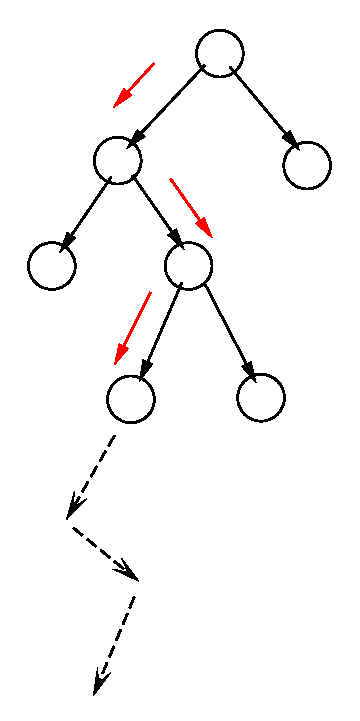
\includegraphics[width=.2\textwidth]{tree.eps}\\
  \caption{A sample game tree in during a UCT search. The red dashed arrow-headed lines represents a search path, including a in-tree part and a play-out simulation part}\label{fig:tree}
\end{figure}

\subsection{Engineering and Some Innovations}

\subsubsection{parallel search structure}
In SuperGo we implemented a simple UCT Search Go framework, equipped with RAVE heuristics a greedy simulator. As more simulations usually results in a more accurate evaluation, SuperGo supports multi-threaded simulations. As the game-tree is a public resource, it should be protected with a lock. ref?? also proposes a lock-free structure that can improve the number of simulations at the cost of some minor inconsistencies, and that structure was employed in Fuego. In our experiments, SuperGo can do about $7000$ simulations in one core. And with two thread running one two cores, we can double the number.

\subsubsection{combining UCT simulations with expert knowledge}
With our observation, UCT search with Monte-Carlo simulation results in a AI player with great overall understanding of the board, but is usually weak in some local, strategic moves. To compensate this, we add expert knowledge with the statistics generated by UCT search when we generate our next move for the game. Originally, after many times of simulation, the AI will select the move corresponding to the child of the tree root with the highest visit-value. Now we multiply visit-value by an additional coefficient, representing how the expert knowledge. For example, we may give a capture move a $1.5$ coefficient, and give a cut move a $1.2$ coefficient.

\subsubsection{different strategies for end game phase}
Monte-Carlo simulation can be quite weak in the open game phase and end game phase. In the open game phase, the visit-value and visit-count of most moves are similar, because there are so many steps



% territory reward

% bias, atari, connect

% dynamic ko

% ----------------------------------------------------------------
